\documentclass[border=9pt]{standalone}
\usepackage[fontset=fandol]{ctex}
\usepackage{amsmath,amssymb,tikz}
\usetikzlibrary{arrows.meta,calc,decorations.pathmorphing}
\tikzset{arr/.style={-{Stealth[length=2mm]},semithick}}
\begin{document}

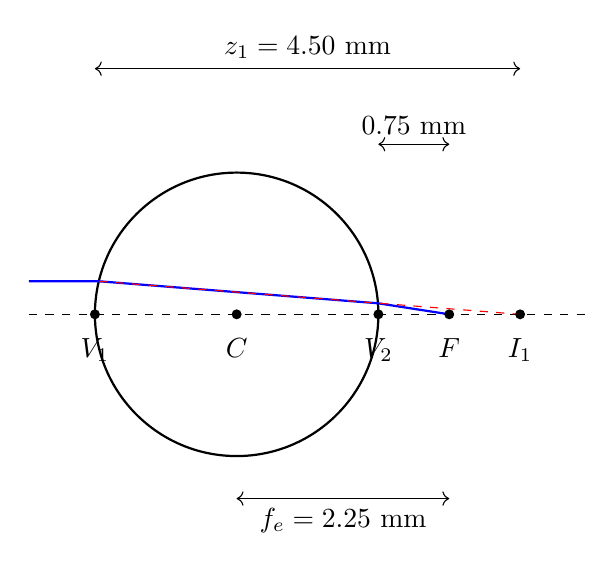
\begin{tikzpicture}[scale=1.2]
\draw[dashed] (-.7,0)--(5.2,0);
\draw[thick] (1.5,0) circle(1.5);
\draw[thick,blue] (-.7,.35)--(.041,.35)--(2.998,.1167)--(3.75,0);
\draw[dashed,red] (.041,.35)--(4.5,0);
\foreach \x/\lab in {0/V_1,1.5/C,3/V_2,3.75/F,4.5/I_1}{
\fill (\x,0) circle(1.5pt); \node[below] at(\x,-.15) {$\lab$};}
\draw[<->] (3,1.8)--(3.75,1.8) node[midway,above] {$0.75\ \mathrm{mm}$};
\draw[<->] (1.5,-1.95)--(3.75,-1.95) node[midway,below] {$f_e=2.25\ \mathrm{mm}$};
\draw[<->] (0,2.6)--(4.5,2.6) node[midway,above] {$z_1=4.50\ \mathrm{mm}$};
\end{tikzpicture}

\end{document}
